\chapter{Redes de comunicación}
En el ámbito informático una red de comunicaciones es representada como una red de ordenadores. Las redes de ordenadores son un conjunto de equipos hardware que están conectados entre sí (ya sea mediante cables o de manera inalámbrica) y que a través de un software especializado envían y reciben impulsos eléctricos (u ondas electromagnética) para el transporte de datos. De esta manera podrán compartir información, recursos u ofrecer servicios.


\section{Breve historia de las redes}
A continuación una breve cronología mostrando los hitos más importantes dentro de las redes de comunicaciones, en lo que a ordenadores se refiere (\href{https://en.wikipedia.org/wiki/Computer_network}{Referencia}).

\begin{description}
    \item[\textasciitilde 1950]
    En la década de los 50 se desarrollan los circuitos integrados. Esto hará que en el futuro los ordenadores cada vez se vayan haciendo más pequeños.

    Las redes de ordenadores comienzan a aparecer en las bases militares americanas, en principio para sistemas de radares.

    \item[\char`\~ 1960]
    Se realiza una conexión entre dos mainframes en EEUU para el sistema de reservas aéreas comerciales.

    El \href{https://es.wikipedia.org/wiki/Instituto_de_Tecnolog%C3%ADa_de_Massachusetts}{MIT} utiliza un ordenador para enrutar y mantener conexiones telefónicas.

    En 1966, aparece un paper (artículo científico) describiendo las WAN.

    En 1969 ARPANET (red de ordenadores creadas por el Departamento de Defensa de Estados Unidos) cuenta con 4 nodos (a 50kbit/s de velocidad).

    \item[\char`\~ 1970]
    En 1972 se hace la primera demostración pública de ARPANET.

    A comienzos de la década (1973) se crea Ethernet en la compañía Xerox Parc.

    A finales de la década Xerox intenta hacer que Ethernet se convierta en un estándar de conexión para terminar con las competencias (token ring, …).

    \begin{center}
        \vspace{-10pt}
        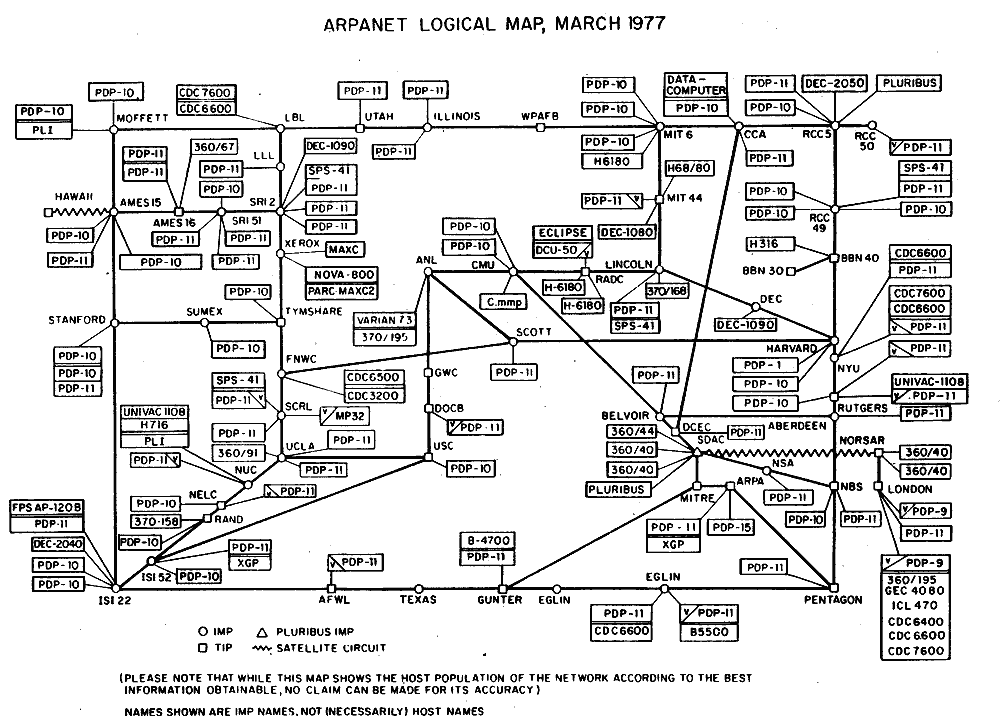
\includegraphics[frame,width=0.9\linewidth]{Arpanet_logical_map_march_1977.png}
        \vspace{-5pt}
        \captionof{figure}{Mapa lógico de ARPANET, marzo de 1977. Origen: \href{https://es.wikipedia.org/wiki/ARPANET\#/media/Archivo:Arpanet_logical_map,_march_1977.png}{ Wikipedia}}\vspace{-13pt}
    \end{center}

    \item[\char`\~ 1980]
    Los ordenadores personales empiezan a generalizarse.

    Aparece el protocolo para enviar y recibir e-mails (SMTP).

    El protocolo TCP/IP se convierte en el utilizado por ARPANET (1983) y es declarado como su estándar para las comunicaciones.

    Aparece el servicio DNS.

    Se crea el modelo de referencia OSI.

    Aparece el primer gusano por la red (Morris worm, 1988). Se estima que infectó al 10\% de los ordenadores conectados a la red.

    Se crea el protocolo BGP.

    El protocolo Ethernet evoluciona y permite conexiones a 10Mbit/s.


    \item[\char`\~ 1990]
    Tim Berners-Lee desarrolla el código para WWW y crea el primer servidor web (1991).

    Se puede decir que aquí es cuando nace la Internet que conocemos actualmente.

    En 1995 Ethernet permite conexiones a 100Mbit/s

    Se establece un control para los nombres de dominio (posteriormente lo asumirá ICANN).

    Aparece Amazon, ebay, Craiglist, IMDB, hotmail, google, yahoo, ...

    Aparece el protocolo IPv6 (1998).

    Aparece el protocolo wifi 802.11b.

    \item[\char`\~ 2000]
    Crisis de las “.com”.

    Internet se generaliza.

    Empiezan a permitirse más TLDs, que no corresponden sólo a países.

    Ethernet permite conexiones a 1Gbit/s

    \item[\char`\~ 2010]
    Ethernet permite conexiones a 400Gbit/s (2018).

    \href{https://en.wikipedia.org/wiki/Starlink}{Starlink} comienza a desplegar su constelación de satélites para dar cobertura en todo el planeta.


\end{description}

\section{Tipos de redes}
A la hora de diferenciar las redes de ordenadores podemos diferenciarlas por distintos conceptos:

\begin{itemize}
    \item Por el medio de transmisión utilizado.
    \item Por la dirección de los datos.
    \item Por el alcance.
    \item Por el grado de acceso.
    \item Por la topología.
    \item ...
\end{itemize}

\subsection{Por el medio de transmisión utilizado}
Más adelante veremos distintos \hyperlink{sistemas_transmision}{sistemas de transmisión}, pero para ir diferenciando podemos crear dos grandes grupos teniendo en cuenta el medio utilizado:

\begin{itemize}
    \item \textbf{Guiados}: Es decir, a través de cables que se encargarn de realizar la transmisión de la señal desde un punto de origen al punto de destino.

    \item \textbf{No guiados}: Se hace uso de algún sistema inalámbrico (mediante antenas) para realizar la transmisión de los datos.
\end{itemize}


\subsection{Por la dirección de los datos}
Si tenemos en cuenta la dirección de los datos en la transmisión, podemos diferenciarlos como:

\begin{itemize}
    \item \textbf{Simplex}: la comunicación sólo se realiza en un único sentido, por lo que sólo es necesario un único canal de transmisión.

    \item \textbf{Half-duplex}: se permite la comunicación en ambos sentidos, pero no de manera simultánea, por lo que emisor y receptor se reparten el tiempo de emisión. Por ejemplo, el \textit{\textbf{walkie-talkie}}.

    \item \textbf{Duplex}: O también conocido como \textit{full-duplex}, permite la comunicación en ambas direcciones y de manera simultánea. Por ejemplo, el \textbf{teléfono}. Para ello es necesario tener una de estas dos opciones:
    \begin{itemize}
        \item Dos canales Half-duplex: uno para cada dirección de la comunicación.
        \item Un único canal por el que se envía la comunicación, pero para ello es necesario algún sistema de multiplexación (como puede ser usar frecuencias separadas).
    \end{itemize}
\end{itemize}


\subsection{Por alcance}
Teniendo en cuenta el alcance al que llegan las redes, podríamos realizar la siguiente distinción:

\subsubsection{Red de área personal (PAN)}
Del inglés \textit{Personal Area Network}, es aquella en la que interactúan distintos dispositivos de muy corto alcance, limitado al área de una persona.

El ejemplo más habitual hoy día sería la comunicación mediante tecnología inalámbrica por Bluetooth en la comunicación entre ordenador, móvil y dispositivos como un \textit{smartwatch}.


\subsubsection{Red de área local (LAN)}
Del inglés \textit{Local Area Network}, es una red que puede abarcar un cierto área de tamaño como una casa, una oficina, un colegio, una universidad...

El ejemplo de una oficina sería una red en la que existen distintos ordenadores, que pueden comunicarse entre sí o compartir información con un servidor ya sea a través de una red cableada o también inalámbrica.

\subsubsection{Red de área metropolitana (MAN)}
Del inglés \textit{Metropolitan Area Network}, y como su nombre indica, el área es mayor y suele abarcar una ciudad para ofrecer los servicios necesarios en la misma.

En este caso también puede ser de manera cableada (normalmente haciendo uso de tecnología más rápida como es la fibra óptica) y también de manera inalámbrica.

Dentro de los servicios que pertenecerían a una MAN podemos poner como ejemplos:
\begin{itemize}
    \item Despliegue de zonas WIFI gratuito en la ciudad.
    \item Comunicación entre sistemas de información (paradas de autobuses, marquesinas, ...).
    \item Sistemas de video-vigilancia municipal.
\end{itemize}

Algunos de estos servicios que están en una MAN pueden ser públicos (como el WIFI) o de acceso restringido (sistemas de seguridad).

\subsubsection{Red de área amplia (WAN)}
Del inglés \textit{Wide Area Network}, es una red que abarca grandes extensiones geográficas y normalmente construidas por grandes empresas o proveedores de internet (ISP, \textit{Internet Service Provider}).


\subsection{Por el grado de acceso}
Teniendo en cuenta quién puede acceder a la red, podríamos definir dos tipos de redes:

\begin{itemize}
    \item \textbf{Red privada}: es una red que sólo ciertas personas pueden acceder y que no normalmente no es accesible desde otras redes. El ejemplo más sencillo es la red que tenemos en casa.
    \item \textbf{Red pública}: es una red a la que puede acceder cualquier persona y que interconecta otras redes sin importar su situación geográfica. Internet es una red pública.
\end{itemize}

%\subsection{Por la topología}
%La topología de una red indica cómo están interconectados los nodos de la misma y el camino que pueden realizar los datos cuando viajan por esa red. En resumen: \textbf{es el diseño de la red}.

%TODO: completar información